\begin{flushright} {\tiny {\color{gray} \tt viscosity\_profile.tex}} \end{flushright}
%~~~~~~~~~~~~~~~~~~~~~~~~~~~~~~~~~~~~~~~~~~~~~~~~~~~~~~~~~~~~~~~~~~~~~~~~~~~~~~~~~~~~~~~~~~~~~~~~~~


\begin{center}
\includegraphics[width=6cm]{images/viscosity_profile/hamy95}\\
{\captionfont \nineteenninetyfive: Taken from Hanyk \etal (1995) \cite{hamy95}. 
$\eta(z)=(1+214.3z\exp-16.7(0.7-z)^2)\times 10^{21}\si{pascal\second}$ }
\end{center}

\begin{center}
\includegraphics[width=6cm]{images/viscosity_profile/csyu97}\\
{\captionfont \nineteenninetyseven: Taken from Cserepes \& Yuen (1997) \cite{csyu97}} 
\end{center}

\begin{center}
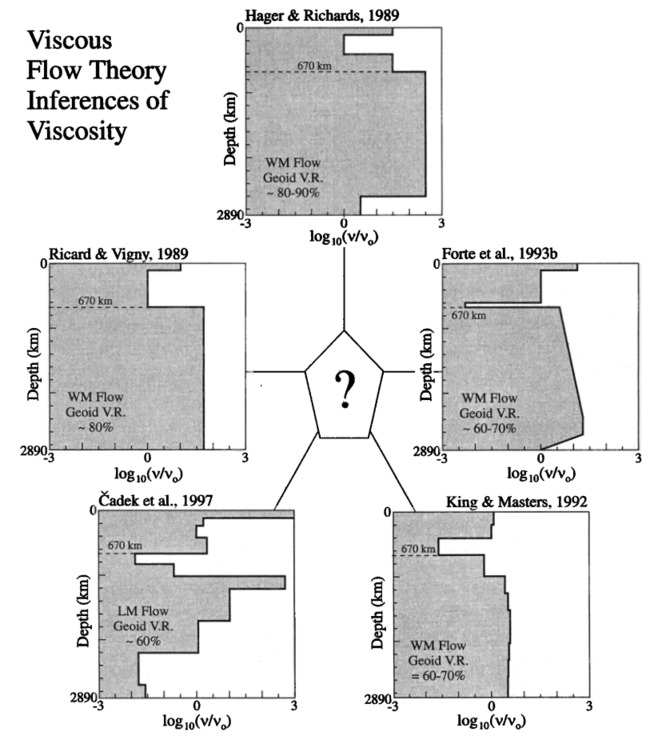
\includegraphics[width=8cm]{images/viscosity_profile/pape98}\\
{\captionfont \nineteenninetyeight: Taken from \textcite{pape98} (1998).} 
\end{center}

\begin{center}
\includegraphics[width=5cm]{images/viscosity_profile/yohk01}\\
{\captionfont \twothousandone:Radial viscosity profile of the reference model. 3-layered model is adopted: 
the lithosphere (0 km to 150 km), the upper mantle (150 km to 670km) 
and the lower mantle (670 km to 2900 km). Taken from \cite{yohk01}}
\end{center}


\begin{center}
\includegraphics[height=6cm]{images/viscosity_profile/profiles_steinberger}
\includegraphics[height=6cm]{images/viscosity_profile/stca06-fig4}\\
{\captionfont \twothousandsix:
Non-optimized, normalized viscosity profiles, as sent by B. Steinberger,
corresponding to fig.~4 in Steinberger \& Calderwood (2006) \cite{stca06}.}
\end{center}

\begin{center}
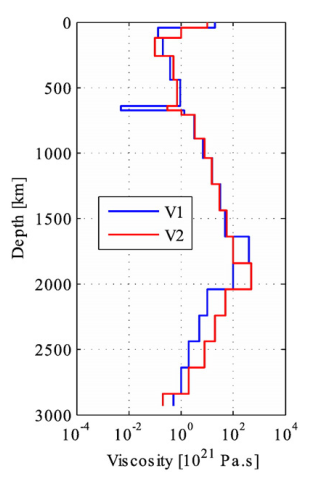
\includegraphics[height=6cm]{images/viscosity_profile/mofm08}\\
{\captionfont Taken from \textcite{mofm08} (2008).}
\end{center}


\begin{center}
\includegraphics[width=11cm]{images/viscosity_profile/capd11}\\
{\captionfont \twothousandeleven: Taken from Cadio \etal \cite{capd11}.
Mantle viscosity structure employed in calculating synthetic geoid anomalies. 
Red: VR (Ricard \etal, 1993); Blue: VMF (Mitrovica and Forte, 2004); Cyan: VMF-LVZ (Mitrovica
and Forte, 2004); Green: VSC (Steinberger and Calderwood, 2006); Orange: VYN (Yoshida and Nakakuki, 2009).}
\end{center}

\begin{center}
\includegraphics[width=11cm]{images/viscosity_profile/civs12-fig1}\\
{\captionfont \twothousandtwelve: Taken from Ciskova \etal \cite{civs12}.}
\end{center}

\begin{center}
\includegraphics[width=6cm]{images/viscosity_profile/kaps14}\\
{\captionfont \twothousandfourteen Taken from Kaban \etal  \cite{kaps14}.
(Black) reference radial viscosity from (Steinberger and Calderwood 2006); 
(Blue) alternative viscosity model of Kaban and Trubitsyn (2012); 
(Light Grey) limits of viscosity variations in the model with LVV (Petrunin \etal 2013).
}
\end{center}

\begin{center}
\includegraphics[width=14cm]{images/viscosity_profile/profiles}\\
{\captionfont Steinberger (2016) \cite{stei16}; 
Ciskova \etal (2012) \cite{civs12}.}
\end{center}

\begin{center}
\includegraphics[width=5cm]{images/viscosity_profile/kani19}\\
{\captionfont \twothousandnineteen: Taken from Kaneko \etal \cite{kani19} (2019).}
\end{center}

\begin{center}
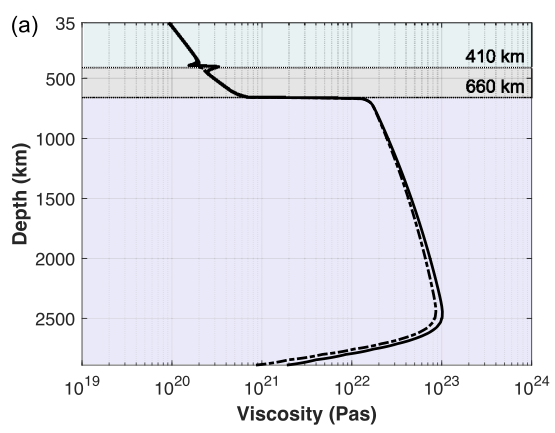
\includegraphics[width=6cm]{images/viscosity_profile/nemi23}\\
{\captionfont \twothousandtwentythree: Taken from \textcite{nemi23} (2023).}
\end{center}

\begin{center}
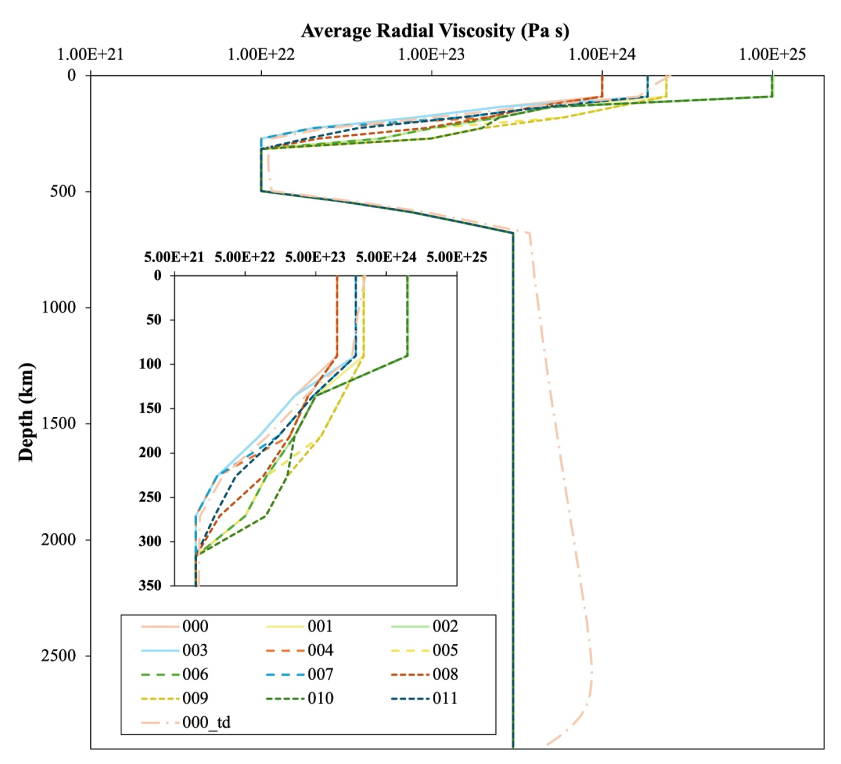
\includegraphics[width=10cm]{images/viscosity_profile/pldp24}\\
{\captionfont \twothousandtwentyfour: Taken from \textcite{pldp24} (2024).}
\end{center}



\Literature:
\begin{itemize} 
\item \fullcite{elss85}
\item \fullcite{mayw11}
\item \fullcite{flam19}
\item \fullcite{mifo04}
\item \fullcite{kima92}
\item \fullcite{rull15}
\item \fullcite{stho08}
\item \fullcite{stei16}
\item \fullcite{cayu93}
\item \fullcite{badw17}
\end{itemize} 
